\documentclass[12pt]{article}

%packages
%\usepackage{latexsym}
\usepackage{graphicx}
\usepackage{color}
\usepackage{amsmath}
\usepackage{dsfont}
\usepackage{placeins}
\usepackage{amssymb}
\usepackage{wasysym}
\usepackage{abstract}
\usepackage{hyperref}
\usepackage{etoolbox}
\usepackage{datetime}
\usepackage{xcolor}
\usepackage{alphalph}
\settimeformat{ampmtime}

%\usepackage{pstricks,pst-node,pst-tree}

%\usepackage{algpseudocode}
%\usepackage{amsthm}
%\usepackage{hyperref}
%\usepackage{mathrsfs}
%\usepackage{amsfonts}
%\usepackage{bbding}
%\usepackage{listings}
%\usepackage{appendix}
\usepackage[margin=1in]{geometry}
%\geometry{papersize={8.5in,11in},total={6.5in,9in}}
%\usepackage{cancel}
%\usepackage{algorithmic, algorithm}

\makeatletter
\def\maxwidth{ %
  \ifdim\Gin@nat@width>\linewidth
    \linewidth
  \else
    \Gin@nat@width
  \fi
}
\makeatother

\definecolor{fgcolor}{rgb}{0.345, 0.345, 0.345}
\newcommand{\hlnum}[1]{\textcolor[rgb]{0.686,0.059,0.569}{#1}}%
\newcommand{\hlstr}[1]{\textcolor[rgb]{0.192,0.494,0.8}{#1}}%
\newcommand{\hlcom}[1]{\textcolor[rgb]{0.678,0.584,0.686}{\textit{#1}}}%
\newcommand{\hlopt}[1]{\textcolor[rgb]{0,0,0}{#1}}%
\newcommand{\hlstd}[1]{\textcolor[rgb]{0.345,0.345,0.345}{#1}}%
\newcommand{\hlkwa}[1]{\textcolor[rgb]{0.161,0.373,0.58}{\textbf{#1}}}%
\newcommand{\hlkwb}[1]{\textcolor[rgb]{0.69,0.353,0.396}{#1}}%
\newcommand{\hlkwc}[1]{\textcolor[rgb]{0.333,0.667,0.333}{#1}}%
\newcommand{\hlkwd}[1]{\textcolor[rgb]{0.737,0.353,0.396}{\textbf{#1}}}%

\usepackage{framed}
\makeatletter
\newenvironment{kframe}{%
 \def\at@end@of@kframe{}%
 \ifinner\ifhmode%
  \def\at@end@of@kframe{\end{minipage}}%
  \begin{minipage}{\columnwidth}%
 \fi\fi%
 \def\FrameCommand##1{\hskip\@totalleftmargin \hskip-\fboxsep
 \colorbox{shadecolor}{##1}\hskip-\fboxsep
     % There is no \\@totalrightmargin, so:
     \hskip-\linewidth \hskip-\@totalleftmargin \hskip\columnwidth}%
 \MakeFramed {\advance\hsize-\width
   \@totalleftmargin\z@ \linewidth\hsize
   \@setminipage}}%
 {\par\unskip\endMakeFramed%
 \at@end@of@kframe}
\makeatother

\definecolor{shadecolor}{rgb}{.77, .77, .77}
\definecolor{messagecolor}{rgb}{0, 0, 0}
\definecolor{warningcolor}{rgb}{1, 0, 1}
\definecolor{errorcolor}{rgb}{1, 0, 0}
\newenvironment{knitrout}{}{} % an empty environment to be redefined in TeX

\usepackage{alltt}
\usepackage[T1]{fontenc}

\newcommand{\qu}[1]{``#1''}
\newcounter{probnum}
\setcounter{probnum}{1}

%create definition to allow local margin changes
\def\changemargin#1#2{\list{}{\rightmargin#2\leftmargin#1}\item[]}
\let\endchangemargin=\endlist 

%allow equations to span multiple pages
\allowdisplaybreaks

%define colors and color typesetting conveniences
\definecolor{gray}{rgb}{0.5,0.5,0.5}
\definecolor{black}{rgb}{0,0,0}
\definecolor{white}{rgb}{1,1,1}
\definecolor{blue}{rgb}{0.5,0.5,1}
\newcommand{\inblue}[1]{\color{blue}#1 \color{black}}
\definecolor{green}{rgb}{0.133,0.545,0.133}
\newcommand{\ingreen}[1]{\color{green}#1 \color{black}}
\definecolor{yellow}{rgb}{1,1,0}
\newcommand{\inyellow}[1]{\color{yellow}#1 \color{black}}
\definecolor{orange}{rgb}{0.9,0.649,0}
\newcommand{\inorange}[1]{\color{orange}#1 \color{black}}
\definecolor{red}{rgb}{1,0.133,0.133}
\newcommand{\inred}[1]{\color{red}#1 \color{black}}
\definecolor{purple}{rgb}{0.58,0,0.827}
\newcommand{\inpurple}[1]{\color{purple}#1 \color{black}}
\definecolor{backgcode}{rgb}{0.97,0.97,0.8}
\definecolor{Brown}{cmyk}{0,0.81,1,0.60}
\definecolor{OliveGreen}{cmyk}{0.64,0,0.95,0.40}
\definecolor{CadetBlue}{cmyk}{0.62,0.57,0.23,0}

%define new math operators
\DeclareMathOperator*{\argmax}{arg\,max~}
\DeclareMathOperator*{\argmin}{arg\,min~}
\DeclareMathOperator*{\argsup}{arg\,sup~}
\DeclareMathOperator*{\arginf}{arg\,inf~}
\DeclareMathOperator*{\convolution}{\text{\Huge{$\ast$}}}
\newcommand{\infconv}[2]{\convolution^\infty_{#1 = 1} #2}
%true functions

%%%% GENERAL SHORTCUTS

%shortcuts for pure typesetting conveniences
\newcommand{\bv}[1]{\boldsymbol{#1}}

%shortcuts for compound constants
\newcommand{\BetaDistrConst}{\dfrac{\Gamma(\alpha + \beta)}{\Gamma(\alpha)\Gamma(\beta)}}
\newcommand{\NormDistrConst}{\dfrac{1}{\sqrt{2\pi\sigma^2}}}

%shortcuts for conventional symbols
\newcommand{\tsq}{\tau^2}
\newcommand{\tsqh}{\hat{\tau}^2}
\newcommand{\sigsq}{\sigma^2}
\newcommand{\sigsqsq}{\parens{\sigma^2}^2}
\newcommand{\sigsqovern}{\dfrac{\sigsq}{n}}
\newcommand{\tausq}{\tau^2}
\newcommand{\tausqalpha}{\tau^2_\alpha}
\newcommand{\tausqbeta}{\tau^2_\beta}
\newcommand{\tausqsigma}{\tau^2_\sigma}
\newcommand{\betasq}{\beta^2}
\newcommand{\sigsqvec}{\bv{\sigma}^2}
\newcommand{\sigsqhat}{\hat{\sigma}^2}
\newcommand{\sigsqhatmlebayes}{\sigsqhat_{\text{Bayes, MLE}}}
\newcommand{\sigsqhatmle}[1]{\sigsqhat_{#1, \text{MLE}}}
\newcommand{\bSigma}{\bv{\Sigma}}
\newcommand{\bSigmainv}{\bSigma^{-1}}
\newcommand{\thetavec}{\bv{\theta}}
\newcommand{\thetahat}{\hat{\theta}}
\newcommand{\thetahatmle}{\hat{\theta}_{\mathrm{MLE}}}
\newcommand{\thetavechatmle}{\hat{\thetavec}_{\mathrm{MLE}}}
\newcommand{\muhat}{\hat{\mu}}
\newcommand{\musq}{\mu^2}
\newcommand{\muvec}{\bv{\mu}}
\newcommand{\muhatmle}{\muhat_{\text{MLE}}}
\newcommand{\lambdahat}{\hat{\lambda}}
\newcommand{\lambdahatmle}{\lambdahat_{\text{MLE}}}
\newcommand{\etavec}{\bv{\eta}}
\newcommand{\alphavec}{\bv{\alpha}}
\newcommand{\minimaxdec}{\delta^*_{\mathrm{mm}}}
\newcommand{\ybar}{\bar{y}}
\newcommand{\xbar}{\bar{x}}
\newcommand{\Xbar}{\bar{X}}
\newcommand{\phat}{\hat{p}}
\newcommand{\Phat}{\hat{P}}
\newcommand{\Zbar}{\bar{Z}}
\newcommand{\iid}{~{\buildrel iid \over \sim}~}
\newcommand{\inddist}{~{\buildrel ind \over \sim}~}
\newcommand{\approxdist}{~{\buildrel approx \over \sim}~}
\newcommand{\equalsindist}{~{\buildrel d \over =}~}
\newcommand{\loglik}[1]{\ell\parens{#1}}
\newcommand{\thetahatkminone}{\thetahat^{(k-1)}}
\newcommand{\thetahatkplusone}{\thetahat^{(k+1)}}
\newcommand{\thetahatk}{\thetahat^{(k)}}
\newcommand{\half}{\frac{1}{2}}
\newcommand{\third}{\frac{1}{3}}
\newcommand{\twothirds}{\frac{2}{3}}
\newcommand{\fourth}{\frac{1}{4}}
\newcommand{\fifth}{\frac{1}{5}}
\newcommand{\sixth}{\frac{1}{6}}

%shortcuts for vector and matrix notation
\newcommand{\A}{\bv{A}}
\newcommand{\At}{\A^T}
\newcommand{\Ainv}{\inverse{\A}}
\newcommand{\B}{\bv{B}}
\newcommand{\K}{\bv{K}}
\newcommand{\Kt}{\K^T}
\newcommand{\Kinv}{\inverse{K}}
\newcommand{\Kinvt}{(\Kinv)^T}
\newcommand{\M}{\bv{M}}
\newcommand{\Bt}{\B^T}
\newcommand{\Q}{\bv{Q}}
\newcommand{\Qt}{\Q^T}
\newcommand{\R}{\bv{R}}
\newcommand{\Rt}{\R^T}
\newcommand{\Z}{\bv{Z}}
\newcommand{\X}{\bv{X}}
\renewcommand{\H}{\bv{H}}
\newcommand{\Xsub}{\X_{\text{(sub)}}}
\newcommand{\Xsubadj}{\X_{\text{(sub,adj)}}}
\newcommand{\I}{\bv{I}}
\newcommand{\Y}{\bv{Y}}
\newcommand{\sigsqI}{\sigsq\I}
\renewcommand{\P}{\bv{P}}
\newcommand{\Psub}{\P_{\text{(sub)}}}
\newcommand{\Pt}{\P^T}
\newcommand{\Pii}{P_{ii}}
\newcommand{\Pij}{P_{ij}}
\newcommand{\IminP}{(\I-\P)}
\newcommand{\Xt}{\bv{X}^T}
\newcommand{\XtX}{\Xt\X}
\newcommand{\XtXinv}{\parens{\Xt\X}^{-1}}
\newcommand{\XtXinvXt}{\XtXinv\Xt}
\newcommand{\XXtXinvXt}{\X\XtXinvXt}
\newcommand{\x}{\bv{x}}
\renewcommand{\b}{\bv{b}}
\newcommand{\onevec}{\bv{1}}
\newcommand{\oneton}{1, \ldots, n}
\newcommand{\yoneton}{y_1, \ldots, y_n}
\newcommand{\yonetonorder}{y_{(1)}, \ldots, y_{(n)}}
\newcommand{\Yoneton}{Y_1, \ldots, Y_n}
\newcommand{\iinoneton}{i \in \braces{\oneton}}
\newcommand{\onetom}{1, \ldots, m}
\newcommand{\jinonetom}{j \in \braces{\onetom}}
\newcommand{\xoneton}{x_1, \ldots, x_n}
\newcommand{\Xoneton}{X_1, \ldots, X_n}
\newcommand{\xt}{\x^T}
\newcommand{\y}{\bv{y}}
\newcommand{\yt}{\y^T}
\renewcommand{\c}{\bv{c}}
\newcommand{\ct}{\c^T}
\newcommand{\tstar}{\bv{t}^*}
\renewcommand{\u}{\bv{u}}
\renewcommand{\v}{\bv{v}}
\renewcommand{\a}{\bv{a}}
\newcommand{\s}{\bv{s}}
\newcommand{\yadj}{\y_{\text{(adj)}}}
\newcommand{\xjadj}{\x_{j\text{(adj)}}}
\newcommand{\xjadjM}{\x_{j \perp M}}
\newcommand{\yhat}{\hat{\y}}
\newcommand{\yhatsub}{\yhat_{\text{(sub)}}}
\newcommand{\yhatstar}{\yhat^*}
\newcommand{\yhatstarnew}{\yhatstar_{\text{new}}}
\newcommand{\z}{\bv{z}}
\newcommand{\zt}{\z^T}
\newcommand{\bb}{\bv{b}}
\newcommand{\bbt}{\bb^T}
\newcommand{\bbeta}{\bv{\beta}}
\newcommand{\beps}{\bv{\epsilon}}
\newcommand{\bepst}{\beps^T}
\newcommand{\e}{\bv{e}}
\newcommand{\Mofy}{\M(\y)}
\newcommand{\KofAlpha}{K(\alpha)}
\newcommand{\ellset}{\mathcal{L}}
\newcommand{\oneminalph}{1-\alpha}
\newcommand{\SSE}{\text{SSE}}
\newcommand{\SSEsub}{\text{SSE}_{\text{(sub)}}}
\newcommand{\MSE}{\text{MSE}}
\newcommand{\RMSE}{\text{RMSE}}
\newcommand{\SSR}{\text{SSR}}
\newcommand{\SST}{\text{SST}}
\newcommand{\JSest}{\delta_{\text{JS}}(\x)}
\newcommand{\Bayesest}{\delta_{\text{Bayes}}(\x)}
\newcommand{\EmpBayesest}{\delta_{\text{EmpBayes}}(\x)}
\newcommand{\BLUPest}{\delta_{\text{BLUP}}}
\newcommand{\MLEest}[1]{\hat{#1}_{\text{MLE}}}

%shortcuts for Linear Algebra stuff (i.e. vectors and matrices)
\newcommand{\twovec}[2]{\bracks{\begin{array}{c} #1 \\ #2 \end{array}}}
\newcommand{\threevec}[3]{\bracks{\begin{array}{c} #1 \\ #2 \\ #3 \end{array}}}
\newcommand{\fivevec}[5]{\bracks{\begin{array}{c} #1 \\ #2 \\ #3 \\ #4 \\ #5 \end{array}}}
\newcommand{\twobytwomat}[4]{\bracks{\begin{array}{cc} #1 & #2 \\ #3 & #4 \end{array}}}
\newcommand{\threebytwomat}[6]{\bracks{\begin{array}{cc} #1 & #2 \\ #3 & #4 \\ #5 & #6 \end{array}}}

%shortcuts for conventional compound symbols
\newcommand{\thetainthetas}{\theta \in \Theta}
\newcommand{\reals}{\mathbb{R}}
\newcommand{\complexes}{\mathbb{C}}
\newcommand{\rationals}{\mathbb{Q}}
\newcommand{\integers}{\mathbb{Z}}
\newcommand{\naturals}{\mathbb{N}}
\newcommand{\forallninN}{~~\forall n \in \naturals}
\newcommand{\forallxinN}[1]{~~\forall #1 \in \reals}
\newcommand{\matrixdims}[2]{\in \reals^{\,#1 \times #2}}
\newcommand{\inRn}[1]{\in \reals^{\,#1}}
\newcommand{\mathimplies}{\quad\Rightarrow\quad}
\newcommand{\mathlogicequiv}{\quad\Leftrightarrow\quad}
\newcommand{\eqncomment}[1]{\quad \text{(#1)}}
\newcommand{\limitn}{\lim_{n \rightarrow \infty}}
\newcommand{\limitN}{\lim_{N \rightarrow \infty}}
\newcommand{\limitd}{\lim_{d \rightarrow \infty}}
\newcommand{\limitt}{\lim_{t \rightarrow \infty}}
\newcommand{\limitsupn}{\limsup_{n \rightarrow \infty}~}
\newcommand{\limitinfn}{\liminf_{n \rightarrow \infty}~}
\newcommand{\limitk}{\lim_{k \rightarrow \infty}}
\newcommand{\limsupn}{\limsup_{n \rightarrow \infty}}
\newcommand{\limsupk}{\limsup_{k \rightarrow \infty}}
\newcommand{\floor}[1]{\left\lfloor #1 \right\rfloor}
\newcommand{\ceil}[1]{\left\lceil #1 \right\rceil}

%shortcuts for environments
\newcommand{\beqn}{\vspace{-0.25cm}\begin{eqnarray*}}
\newcommand{\eeqn}{\end{eqnarray*}}
\newcommand{\bneqn}{\vspace{-0.25cm}\begin{eqnarray}}
\newcommand{\eneqn}{\end{eqnarray}}

%shortcuts for mini environments
\newcommand{\parens}[1]{\left(#1\right)}
\newcommand{\squared}[1]{\parens{#1}^2}
\newcommand{\tothepow}[2]{\parens{#1}^{#2}}
\newcommand{\prob}[1]{\mathbb{P}\parens{#1}}
\newcommand{\cprob}[2]{\prob{#1~|~#2}}
\newcommand{\littleo}[1]{o\parens{#1}}
\newcommand{\bigo}[1]{O\parens{#1}}
\newcommand{\Lp}[1]{\mathbb{L}^{#1}}
\renewcommand{\arcsin}[1]{\text{arcsin}\parens{#1}}
\newcommand{\prodonen}[2]{\bracks{\prod_{#1=1}^n #2}}
\newcommand{\mysum}[4]{\sum_{#1=#2}^{#3} #4}
\newcommand{\sumonen}[2]{\sum_{#1=1}^n #2}
\newcommand{\infsum}[2]{\sum_{#1=1}^\infty #2}
\newcommand{\infprod}[2]{\prod_{#1=1}^\infty #2}
\newcommand{\infunion}[2]{\bigcup_{#1=1}^\infty #2}
\newcommand{\infinter}[2]{\bigcap_{#1=1}^\infty #2}
\newcommand{\infintegral}[2]{\int^\infty_{-\infty} #2 ~\text{d}#1}
\newcommand{\supthetas}[1]{\sup_{\thetainthetas}\braces{#1}}
\newcommand{\bracks}[1]{\left[#1\right]}
\newcommand{\braces}[1]{\left\{#1\right\}}
\newcommand{\set}[1]{\left\{#1\right\}}
\newcommand{\abss}[1]{\left|#1\right|}
\newcommand{\norm}[1]{\left|\left|#1\right|\right|}
\newcommand{\normsq}[1]{\norm{#1}^2}
\newcommand{\inverse}[1]{\parens{#1}^{-1}}
\newcommand{\rowof}[2]{\parens{#1}_{#2\cdot}}

%shortcuts for functionals
\newcommand{\realcomp}[1]{\text{Re}\bracks{#1}}
\newcommand{\imagcomp}[1]{\text{Im}\bracks{#1}}
\newcommand{\range}[1]{\text{range}\bracks{#1}}
\newcommand{\colsp}[1]{\text{colsp}\bracks{#1}}
\newcommand{\rowsp}[1]{\text{rowsp}\bracks{#1}}
\newcommand{\tr}[1]{\text{tr}\bracks{#1}}
\newcommand{\rank}[1]{\text{rank}\bracks{#1}}
\newcommand{\proj}[2]{\text{Proj}_{#1}\bracks{#2}}
\newcommand{\projcolspX}[1]{\text{Proj}_{\colsp{\X}}\bracks{#1}}
\newcommand{\median}[1]{\text{median}\bracks{#1}}
\newcommand{\mean}[1]{\text{mean}\bracks{#1}}
\newcommand{\dime}[1]{\text{dim}\bracks{#1}}
\renewcommand{\det}[1]{\text{det}\bracks{#1}}
\newcommand{\expe}[1]{\mathbb{E}\bracks{#1}}
\newcommand{\expeabs}[1]{\expe{\abss{#1}}}
\newcommand{\expesub}[2]{\mathbb{E}_{#1}\bracks{#2}}
\newcommand{\indic}[1]{\mathds{1}_{#1}}
\newcommand{\var}[1]{\mathbb{V}\text{ar}\bracks{#1}}
\newcommand{\cov}[2]{\mathbb{C}\text{ov}\bracks{#1, #2}}
\newcommand{\corr}[2]{\text{Corr}\bracks{#1, #2}}
\newcommand{\se}[1]{\mathbb{S}\text{E}\bracks{#1}}
\newcommand{\seest}[1]{\hat{\mathbb{S}\text{E}}\bracks{#1}}
\newcommand{\bias}[1]{\text{Bias}\bracks{#1}}
\newcommand{\derivop}[2]{\dfrac{\text{d}}{\text{d} #1}\bracks{#2}}
\newcommand{\partialop}[2]{\dfrac{\partial}{\partial #1}\bracks{#2}}
\newcommand{\secpartialop}[2]{\dfrac{\partial^2}{\partial #1^2}\bracks{#2}}
\newcommand{\mixpartialop}[3]{\dfrac{\partial^2}{\partial #1 \partial #2}\bracks{#3}}

%shortcuts for functions
\renewcommand{\exp}[1]{\mathrm{exp}\parens{#1}}
\renewcommand{\cos}[1]{\text{cos}\parens{#1}}
\renewcommand{\sin}[1]{\text{sin}\parens{#1}}
\newcommand{\sign}[1]{\text{sign}\parens{#1}}
\newcommand{\are}[1]{\mathrm{ARE}\parens{#1}}
\newcommand{\natlog}[1]{\ln\parens{#1}}
\newcommand{\oneover}[1]{\frac{1}{#1}}
\newcommand{\overtwo}[1]{\frac{#1}{2}}
\newcommand{\overn}[1]{\frac{#1}{n}}
\newcommand{\oneoversqrt}[1]{\oneover{\sqrt{#1}}}
\newcommand{\sqd}[1]{\parens{#1}^2}
\newcommand{\loss}[1]{\ell\parens{\theta, #1}}
\newcommand{\losstwo}[2]{\ell\parens{#1, #2}}
\newcommand{\cf}{\phi(t)}

%English language specific shortcuts
\newcommand{\ie}{\textit{i.e.} }
\newcommand{\AKA}{\textit{AKA} }
\renewcommand{\iff}{\textit{iff}}
\newcommand{\eg}{\textit{e.g.} }
\newcommand{\st}{\textit{s.t.} }
\newcommand{\wrt}{\textit{w.r.t.} }
\newcommand{\mathst}{~~\text{\st}~~}
\newcommand{\mathand}{~~\text{and}~~}
\newcommand{\ala}{\textit{a la} }
\newcommand{\ppp}{posterior predictive p-value}
\newcommand{\dd}{dataset-to-dataset}

%shortcuts for distribution titles
\newcommand{\logistic}[2]{\mathrm{Logistic}\parens{#1,\,#2}}
\newcommand{\bernoulli}[1]{\mathrm{Bernoulli}\parens{#1}}
\newcommand{\betanot}[2]{\mathrm{Beta}\parens{#1,\,#2}}
\newcommand{\stdbetanot}{\betanot{\alpha}{\beta}}
\newcommand{\multnormnot}[3]{\mathcal{N}_{#1}\parens{#2,\,#3}}
\newcommand{\normnot}[2]{\mathcal{N}\parens{#1,\,#2}}
\newcommand{\classicnormnot}{\normnot{\mu}{\sigsq}}
\newcommand{\stdnormnot}{\normnot{0}{1}}
\newcommand{\uniformdiscrete}[1]{\mathrm{Uniform}\parens{\braces{#1}}}
\newcommand{\uniform}[2]{\mathrm{U}\parens{#1,\,#2}}
\newcommand{\stduniform}{\uniform{0}{1}}
\newcommand{\geometric}[1]{\mathrm{Geometric}\parens{#1}}
\newcommand{\hypergeometric}[3]{\mathrm{Hypergeometric}\parens{#1,\,#2,\,#3}}
\newcommand{\exponential}[1]{\mathrm{Exp}\parens{#1}}
\newcommand{\gammadist}[2]{\mathrm{Gamma}\parens{#1, #2}}
\newcommand{\poisson}[1]{\mathrm{Poisson}\parens{#1}}
\newcommand{\binomial}[2]{\mathrm{Binomial}\parens{#1,\,#2}}
\newcommand{\negbin}[2]{\mathrm{NegBin}\parens{#1,\,#2}}
\newcommand{\rayleigh}[1]{\mathrm{Rayleigh}\parens{#1}}
\newcommand{\multinomial}[2]{\mathrm{Multinomial}\parens{#1,\,#2}}
\newcommand{\gammanot}[2]{\mathrm{Gamma}\parens{#1,\,#2}}
\newcommand{\cauchynot}[2]{\text{Cauchy}\parens{#1,\,#2}}
\newcommand{\invchisqnot}[1]{\text{Inv}\chisq{#1}}
\newcommand{\invscaledchisqnot}[2]{\text{ScaledInv}\ncchisq{#1}{#2}}
\newcommand{\invgammanot}[2]{\text{InvGamma}\parens{#1,\,#2}}
\newcommand{\chisq}[1]{\chi^2_{#1}}
\newcommand{\ncchisq}[2]{\chi^2_{#1}\parens{#2}}
\newcommand{\ncF}[3]{F_{#1,#2}\parens{#3}}

%shortcuts for PDF's of common distributions
\newcommand{\logisticpdf}[3]{\oneover{#3}\dfrac{\exp{-\dfrac{#1 - #2}{#3}}}{\parens{1+\exp{-\dfrac{#1 - #2}{#3}}}^2}}
\newcommand{\betapdf}[3]{\dfrac{\Gamma(#2 + #3)}{\Gamma(#2)\Gamma(#3)}#1^{#2-1} (1-#1)^{#3-1}}
\newcommand{\normpdf}[3]{\frac{1}{\sqrt{2\pi#3}}\exp{-\frac{1}{2#3}(#1 - #2)^2}}
\newcommand{\normpdfvarone}[2]{\dfrac{1}{\sqrt{2\pi}}e^{-\half(#1 - #2)^2}}
\newcommand{\chisqpdf}[2]{\dfrac{1}{2^{#2/2}\Gamma(#2/2)}\; {#1}^{#2/2-1} e^{-#1/2}}
\newcommand{\invchisqpdf}[2]{\dfrac{2^{-\overtwo{#1}}}{\Gamma(#2/2)}\,{#1}^{-\overtwo{#2}-1}  e^{-\oneover{2 #1}}}
\newcommand{\exponentialpdf}[2]{#2\exp{-#2#1}}
\newcommand{\poissonpdf}[2]{\dfrac{e^{-#1} #1^{#2}}{#2!}}
\newcommand{\binomialpdf}[3]{\binom{#2}{#1}#3^{#1}(1-#3)^{#2-#1}}
\newcommand{\rayleighpdf}[2]{\dfrac{#1}{#2^2}\exp{-\dfrac{#1^2}{2 #2^2}}}
\newcommand{\gammapdf}[3]{\dfrac{#3^#2}{\Gamma\parens{#2}}#1^{#2-1}\exp{-#3 #1}}
\newcommand{\cauchypdf}[3]{\oneover{\pi} \dfrac{#3}{\parens{#1-#2}^2 + #3^2}}
\newcommand{\Gammaf}[1]{\Gamma\parens{#1}}

%shortcuts for miscellaneous typesetting conveniences
\newcommand{\notesref}[1]{\marginpar{\color{gray}\tt #1\color{black}}}

%%%% DOMAIN-SPECIFIC SHORTCUTS

%Real analysis related shortcuts
\newcommand{\zeroonecl}{\bracks{0,1}}
\newcommand{\forallepsgrzero}{\forall \epsilon > 0~~}
\newcommand{\lessthaneps}{< \epsilon}
\newcommand{\fraccomp}[1]{\text{frac}\bracks{#1}}

%Bayesian related shortcuts
\newcommand{\yrep}{y^{\text{rep}}}
\newcommand{\yrepisq}{(\yrep_i)^2}
\newcommand{\yrepvec}{\bv{y}^{\text{rep}}}


%Probability shortcuts
\newcommand{\SigField}{\mathcal{F}}
\newcommand{\ProbMap}{\mathcal{P}}
\newcommand{\probtrinity}{\parens{\Omega, \SigField, \ProbMap}}
\newcommand{\convp}{~{\buildrel p \over \rightarrow}~}
\newcommand{\convLp}[1]{~{\buildrel \Lp{#1} \over \rightarrow}~}
\newcommand{\nconvp}{~{\buildrel p \over \nrightarrow}~}
\newcommand{\convae}{~{\buildrel a.e. \over \longrightarrow}~}
\newcommand{\convau}{~{\buildrel a.u. \over \longrightarrow}~}
\newcommand{\nconvau}{~{\buildrel a.u. \over \nrightarrow}~}
\newcommand{\nconvae}{~{\buildrel a.e. \over \nrightarrow}~}
\newcommand{\convd}{~{\buildrel \mathcal{D} \over \rightarrow}~}
\newcommand{\nconvd}{~{\buildrel \mathcal{D} \over \nrightarrow}~}
\newcommand{\withprob}{~~\text{w.p.}~~}
\newcommand{\io}{~~\text{i.o.}}

\newcommand{\Acl}{\bar{A}}
\newcommand{\ENcl}{\bar{E}_N}
\newcommand{\diam}[1]{\text{diam}\parens{#1}}

\newcommand{\taua}{\tau_a}

\newcommand{\myint}[4]{\int_{#2}^{#3} #4 \,\text{d}#1}
\newcommand{\laplacet}[1]{\mathscr{L}\bracks{#1}}
\newcommand{\laplaceinvt}[1]{\mathscr{L}^{-1}\bracks{#1}}
\renewcommand{\min}[1]{\text{min}\braces{#1}}
\renewcommand{\max}[1]{\text{max}\braces{#1}}

\newcommand{\Vbar}[1]{\bar{V}\parens{#1}}
\newcommand{\expnegrtau}{\exp{-r\tau}}

%%% problem typesetting
\definecolor{darkgrey}{rgb}{0.10,0.10,0.9}

\newcommand{\problem}[1]{\noindent \colorbox{black}{{\color{yellow} \large{\textsf{\textbf{Problem \arabic{probnum}}}}~}} \addtocounter{probnum}{1} \vspace{0.2cm} \\ \iftoggle{professormode}{}{\color{darkgrey}} #1}

\newcommand{\easysubproblem}[1]{\ingreen{\item} \iftoggle{professormode}{}{\color{darkgrey}} [easy] #1 \color{black} }
\newcommand{\intermediatesubproblem}[1]{\inorange{\item} \iftoggle{professormode}{}{\color{darkgrey}} [harder] #1 \color{black} }
\newcommand{\hardsubproblem}[1]{\inred{\item} \iftoggle{professormode}{}{\color{darkgrey}} [difficult] #1 \color{black} }
\newcommand{\extracreditsubproblem}[1]{\inpurple{\item} \iftoggle{professormode}{}{\color{darkgrey}} [E.C.] #1 \color{black} }


\newcommand{\spc}[1]{\iftoggle{professormode}{\\ \vspace{#1cm}}{\\ \vspace{-0.3cm}}}

\makeatletter
\newalphalph{\alphmult}[mult]{\@alph}{26}
\renewcommand{\labelenumi}{(\alphmult{\value{enumi}})}

\newcommand{\support}[1]{\text{Supp}\bracks{#1}}
\newcommand{\mode}[1]{\text{Mode}\bracks{#1}}
\newcommand{\IQR}[1]{\text{IQR}\bracks{#1}}
\newcommand{\quantile}[2]{\text{Quantile}\bracks{#1,\,#2}}


\title{Math 342W / 650.4 Spring \the\year \\ Midterm Examination One}
\author{Professor Adam Kapelner}

\date{Thursday, March 14}

\begin{document}
\maketitle

\noindent Full Name \line(1,0){410}

\thispagestyle{empty}

\section*{Code of Academic Integrity}

\footnotesize
Since the college is an academic community, its fundamental purpose is the pursuit of knowledge. Essential to the success of this educational mission is a commitment to the principles of academic integrity. Every member of the college community is responsible for upholding the highest standards of honesty at all times. Students, as members of the community, are also responsible for adhering to the principles and spirit of the following Code of Academic Integrity.

Activities that have the effect or intention of interfering with education, pursuit of knowledge, or fair evaluation of a student's performance are prohibited. Examples of such activities include but are not limited to the following definitions:

\paragraph{Cheating} Using or attempting to use unauthorized assistance, material, or study aids in examinations or other academic work or preventing, or attempting to prevent, another from using authorized assistance, material, or study aids. Example: using an unauthorized cheat sheet in a quiz or exam, altering a graded exam and resubmitting it for a better grade, etc.
\\

\noindent I acknowledge and agree to uphold this Code of Academic Integrity. \\

\begin{center}
\line(1,0){250} ~~~ \line(1,0){100}\\
~~~~~~~~~~~~~~~~~~~~~signature~~~~~~~~~~~~~~~~~~~~~~~~~~~~~~~~~~~~~~~~~~~~~ date
\end{center}

\normalsize

\section*{Instructions}

This exam is 110 minutes and closed-book. You are allowed \textbf{two} pages (front and back) of a \qu{cheat sheet.} You may use a graphing calculator of your choice. Please read the questions carefully. If the question reads \qu{compute,} this means the solution will be a number otherwise you can leave the answer in \textit{any} widely accepted mathematical notation which could be resolved to an exact or approximate number with the use of a computer. I advise you to skip problems marked \qu{[Extra Credit]} until you have finished the other questions on the exam, then loop back and plug in all the holes. I also advise you to use pencil. The exam is 100 points total plus extra credit. Partial credit will be granted for incomplete answers on most of the questions. \fbox{Box} in your final answers. Good luck!

\pagebreak

\problem This question is about modeling in general. \qu{Look both ways before you cross the street} is typical advice. We will attempt to understand this advice from a modeling point of view. There is one feature in this model and one response. Let the response be and feature be:

\beqn
&& y_i := \indic{\text{during street crossing $i$, the person gets hit by a car}} \\
&& x_i  := \indic{\text{during street crossing $i$, the person looks down the street in both directions and does not see any cars coming}} \\
\eeqn

\benum

\subquestionwithpoints{2}  What is the unit in this modeling scenario? \spc{1}

\subquestionwithpoints{1}  What is the data type of $x$? (1 word) \spc{0.5}

\subquestionwithpoints{4}  \qu{Look both ways before you cross the street} implies the following model:\vspace{-0.5cm}

\beqn
\hspace{-4cm}g(x) = 
\eeqn~\vspace{-0.5cm}

\subquestionwithpoints{3}  Describe a scenario where $y \neq g(x)$. \spc{4}

\subquestionwithpoints{3}  Why is this model \qu{wrong but useful}? \spc{4}

\subquestionwithpoints{2}  Is $g$ a mathematical model? Yes / no \spc{-0.5}
\eenum

\problem Consider the following \texttt{R} code from the class demos and labs. The numbers on the right are line numbers that will be referred to later. They are not part of the code.
%,label=R code
\begin{Verbatim}[frame=single,numbers=left]
> y = MASS::Boston$medv
> var(y)
[1] 84.58672
> X = as.matrix(cbind(1, MASS::Boston[, 1 : 13]))
> n = nrow(X)
> n
[1] 506
> Xt = t(X)
> XtX = Xt %*% X
> XtXinv = solve(XtX)
> XtXinvXt = XtXinv %*% Xt
> b = XtXinvXt %*% y
> H = X %*% XtXinvXt
> I_minus_H = diag(n) - H
> yhat = H %*% y
> e = I_minus_H %*% y
> var(e)
         [,1]
[1,] 21.93819
\end{Verbatim}

%Note that $n = 506$. You'll need this fact to answer the questions below.

\benum
\subquestionwithpoints{2} What is returned by \texttt{R} when evaluating \texttt{length(b)}?\spc{0.3}
\subquestionwithpoints{2} What is returned by \texttt{R} when evaluating \texttt{ncol(XtX)}?\spc{0.3}
\subquestionwithpoints{2} What is returned by \texttt{R} when evaluating \texttt{ncol(H)}?\spc{0.3}
\subquestionwithpoints{2} What is returned by \texttt{R} when evaluating \texttt{Matrix::rankMatrix(I\_minus\_H)}?\spc{0.3}
\subquestionwithpoints{3} Compute SST to the nearest two decimals.\spc{1}
\subquestionwithpoints{3} Compute SSE to the nearest two decimals.\spc{1}

Now consider the following scenario: we add random predictors to the design matrix $\X$ one-by-one and run the code above for each updated design matrix $\X$.

\subquestionwithpoints{3} What is the maximum number of random predictors that can be added before the code throws an error and halts? \spc{1}

\subquestionwithpoints{2} If you add too many random predictors, which line number does the code throw this error and halt? \spc{1}

\subquestionwithpoints{5} Graph the expected $R^2$ by number of predictors from 1 to the maximum number that can be considered before OLS fails. Label the x-axis \qu{number of predictors}; label the y-axis \qu{$R^2$}. Graph it to scale. Be sure to mark critical points along both axes.\spc{10} 

Now consider that 10\% of the data was left out in a test set.

\subquestionwithpoints{2} What is the value of $K$?\spc{1}

\subquestionwithpoints{6} Graph expected $oosR^2$ by number of predictors from 1 to the maximum number that can be considered before OLS fails. Label the x-axis \qu{number of predictors}; label the y-axis \qu{$R^2$}. Graph it to scale. Be sure to mark critical points along both axes.\spc{8} 


\eenum



\problem Below is the result of \texttt{skimr::skim} run on the dataset \texttt{ggplot2::diamonds}.


\begin{Verbatim}[frame=single,fontsize=\scriptsize]
-- Data Summary ------------------------
                           Values
Name                       Xy    
Number of rows             53940 
Number of columns          10    
-----------------------          
Column type frequency:           
  factor                   3     
  numeric                  7     
------------------------         
Group variables            None  

-- Variable type: factor ----------------------------------------------------
  skim-variable n-missing complete-rate ordered n-unique top-counts                                   
1 cut                   0             1 TRUE           5 Ide: 21551, Pre: 13791, Ver: 12082, Goo: 4906
2 color                 0             1 TRUE           7 G: 11292, E: 9797, F: 9542, H: 8304          
3 clarity               0             1 TRUE           8 SI1: 13065, VS2: 12258, SI2: 9194, VS1: 8171 

-- Variable type: numeric ----------------------------------------------------
  skim-variable n-missing complete-rate     mean       sd    p0    p25     p50     p75     p100 
1 carat                 0             1    0.798    0.474   0.2   0.4     0.7     1.04     5.01 
2 depth                 0             1   61.7      1.43   43    61      61.8    62.5     79    
3 table                 0             1   57.5      2.23   43    56      57      59       95   
4 price                 0             1 3933.    3989.    326   950    2401    5324.   18823   
5 x                     0             1    5.73     1.12    0     4.71    5.7     6.54    10.7  
6 y                     0             1    5.73     1.14    0     4.72    5.71    6.54    58.9  
7 z                     0             1    3.54     0.706   0     2.91    3.53    4.04    31.8  
\end{Verbatim}



Here is a plot of variable \texttt{cut} by variables \texttt{carat} and \texttt{depth} for a sample of $n_0 = 135$.

\begin{figure}[htp]
\centering
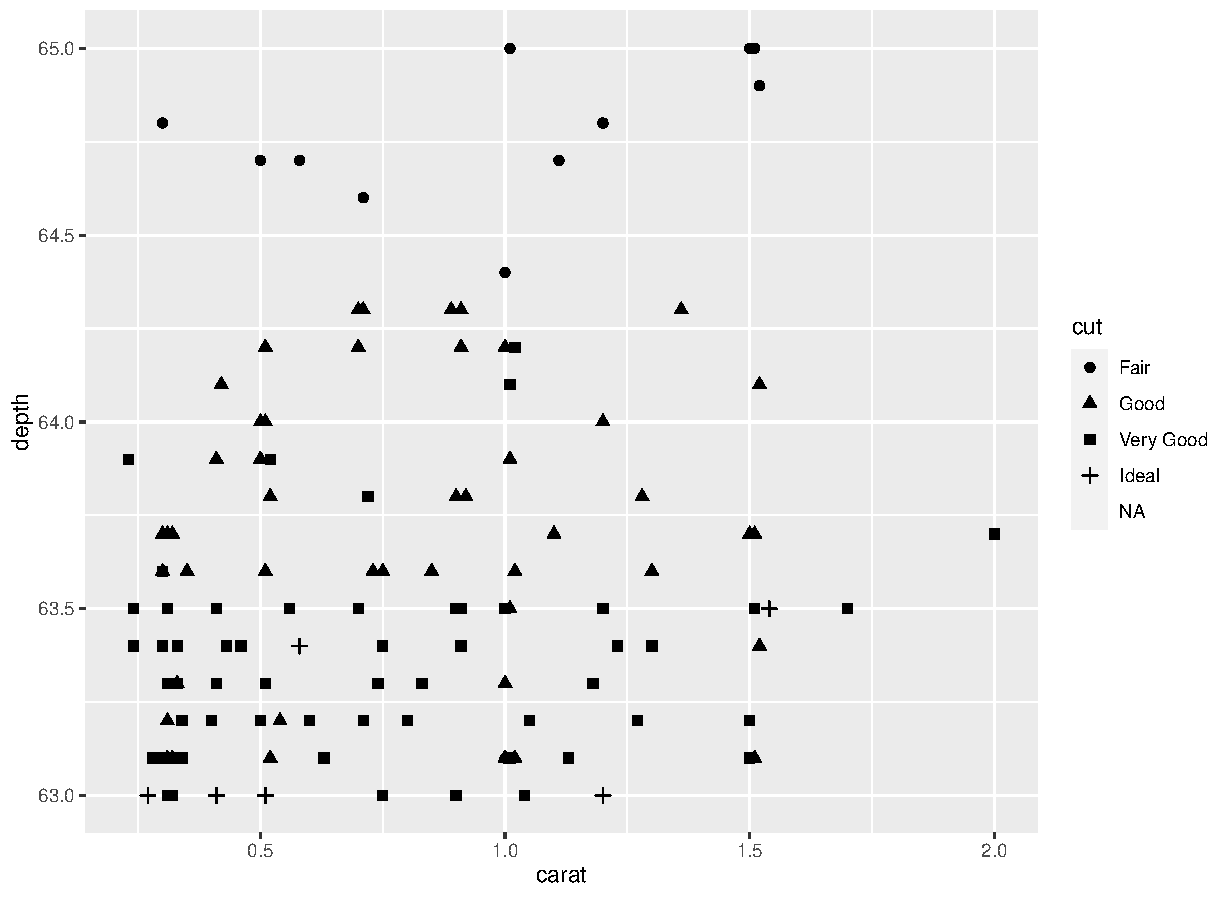
\includegraphics[width=5.9in]{caratdepthcut1}
\end{figure}

\benum

\subquestionwithpoints{2} If we wish to build a model predicting \texttt{cut}, a nominal categorical variable. What type of model is this called? \spc{0}

\subquestionwithpoints{2} Consider all algorithms we studied thus far for this type of response. Regardless of the algorithm employed to create $g$, what would the main source of generalization error be? Your answer must be one of the three sources of error.\spc{0}

\subquestionwithpoints{4} Let \texttt{carat} = 1.6 and \texttt{depth} = 63.5 and let $\mathcal{A}$ be the 6-nearest neighbors algorithm with the Euclidean distance function. Predict $y$.\spc{0}

Consider $\mathbb{D}$ to be only records where \texttt{depth} $\geq$ 64.5. Employ the KNN algorithm with $K=3$ and the Euclidean distance function. 
\subquestionwithpoints{3} What would the in-sample error be? \spc{0.5}

\subquestionwithpoints{4} Use leave-one-out cross validation (i.e. the test set consists of one record for each fold). What would the out of sample error be? \spc{0.5}

We are interested in predicting if a diamond has a cut \qu{more than fair} in the $\mathbb{D}$ plotted below.


\begin{figure}[htp]
\centering
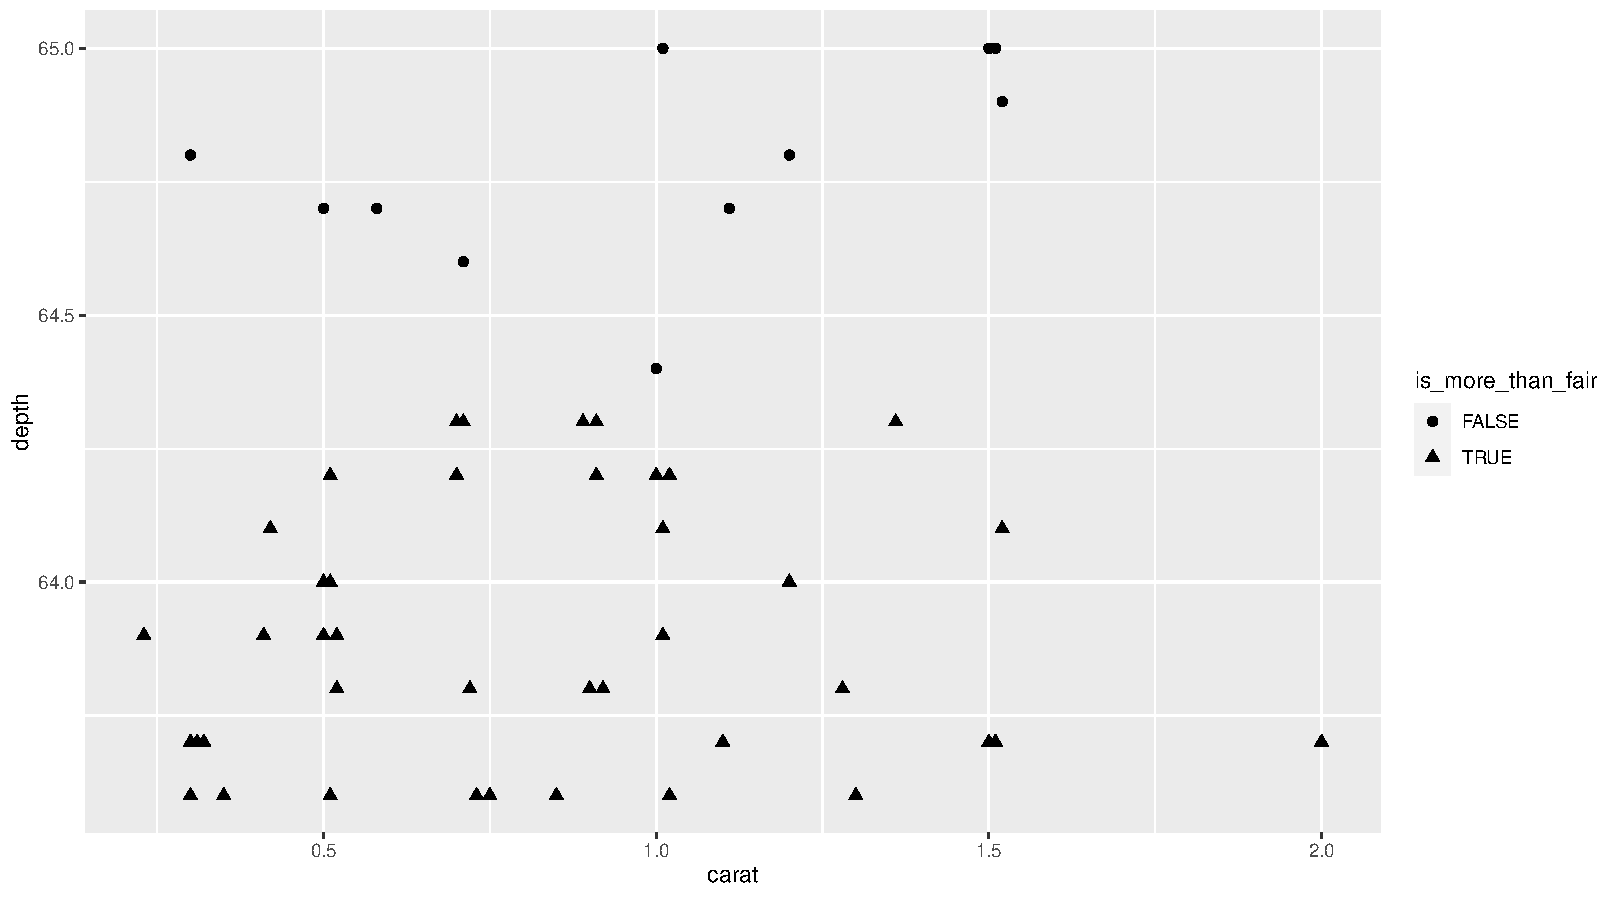
\includegraphics[width=7.0in]{more_than_fair}
\end{figure}

\subquestionwithpoints{2} What type of model is this called? \spc{0}

Circle the following bullet circles which are true:
\subquestionwithpoints{2} \texttt{depth} and \texttt{carat} are likely dependent.\spc{-0.5}
\subquestionwithpoints{2} \texttt{depth} and \texttt{carat} are likely associated.\spc{-0.5}
\subquestionwithpoints{2} \texttt{depth} and \texttt{is\_more\_than\_fair} are likely dependent.\spc{-0.5}
\subquestionwithpoints{2} This dataset is linearly separable.\spc{-0.5}
\subquestionwithpoints{2} If the perceptron is employed, it will converge.  \spc{-0.5}
\subquestionwithpoints{2} Assuming the perceptron algorithm converges, regardless of the starting position, the perceptron will converge to the same place.  \spc{-0.5}
\subquestionwithpoints{2} If the SVM is employed with the Vapnik objective function, the hinge error will be zero.\spc{-0.5}
\subquestionwithpoints{4} The SVM and the perceptron are highly likely to exhibit similar performance for future data that is generated from the same stationary process as $\mathbb{D}$.\spc{-0.5}


\eenum


\problem Assume $\X \in \reals^{n \times (p+1)}$ with $p >1$ composed of random realizations from iid standard normal random variables, full rank. Let $\Q$, $\R$ be the matrix results of the QR-decomposition procedure run on $\X$. Let $\y \in \reals^n$ which a vector of measurements of a phenomenon of interest.  %Let $\e$ denote the vector of in-sample residuals where $\e \neq \y$ and $\sum_{i=1}^n e_i^2 \neq 0$.

\benum
\subquestionwithpoints{10} Prove that the $\normsq{\Q\Q^\top\y} \Big/ \normsq{\y} \in \zeroonecl$. \spc{13} 


\subquestionwithpoints{2} If you were to use $\mathcal{A} =$ OLS to generate $g$, which of the three sources of error would be the main source of error in $g$? \spc{1} 

Circle the following bullet circles which are true:
\subquestionwithpoints{2} $\exists c \neq 0$ s.t. $\X_{\cdot 1} = c\,\Q_{\cdot 1}$. \spc{-0.5}
\subquestionwithpoints{2} $\exists c \neq 0$ s.t. $\X_{\cdot 2} = c\,\Q_{\cdot 2}$. \spc{-0.5}
\subquestionwithpoints{2} $\colsp{\R} =\colsp{\X}$. \spc{-0.5}
\eenum

\end{document}

\problem This question is about science and modeling in general.

\benum
\subquestionwithpoints{4} When an object free falls to the ground from height $h$, an elementary physics provides textbook provides the formula for the predicted time $t$ the object takes to reach the ground as $t = \sqrt{2h/g}$ where $g$ is a constant. Explain why this formula is \qu{wrong but useful}.\spc{4}

\subquestionwithpoints{9} Circle the letters of all the following that are \textbf{true}.

\begin{enumerate}[(a)]
\item A \qu{phenomenon} is anything one finds interesting in the world
\item The enterprise of the scientific endeavor is essentially modeling
\item The two goals of modeling is to provide predictions of the phenomenon in future settings and explanation of how the settings affect the phenomenon 
\item Two different people can come to two different predictions for the same observation using a non-mathematical model
\item Given one mathematical model $g$, there can be two different $y$ values for equal $\x$ input vectors
\item Given one mathematical model $g$, there can be two different $\hat{y}$ values for equal $\x$ input vectors
\item The naive model $g-0$ requires historical data
\item The naive model $g-0$ can be used for prediction
\item The naive model $g-0$ cannot be validated since it does not make use of the $\x-{i\cdot}$'s

\end{enumerate}

\subquestionwithpoints{6} Circle the letters of all the following that are \textbf{true}. In the quote by George Box and Norman Draper in 1987, \qu{All models are wrong but some are useful} means that models ...


\begin{enumerate}[(a)]
\item ... must have univariate response
\item ... must be constructed using supervised learning
\item ... sometimes provide accuracy that meets your prediction goals
\item ... never can achieve perfect predictive accuracy
\item ... need perfectly accurate input measurements
\item ... never describe the pheonomenon absolutely
\end{enumerate}

\eenum


\problem Consider the diamonds dataset which is part of the \texttt{ggplot2} package in \texttt{R}. This is a dataset we will be looking at extensively later in the course.

\begin{lstlisting}
> D = ggplot2::diamonds
> dim(D)
[1] 53940    10
> summary(D)
     carat               cut        color        clarity     
 Min.   :0.2000   Fair     : 1610   D: 6775   SI1    :13065  
 1st Qu.:0.4000   Good     : 4906   E: 9797   VS2    :12258  
 Median :0.7000   Very Good:12082   F: 9542   SI2    : 9194  
 Mean   :0.7979   Premium  :13791   G:11292   VS1    : 8171  
 3rd Qu.:1.0400   Ideal    :21551   H: 8304   VVS2   : 5066  
 Max.   :5.0100                     I: 5422   VVS1   : 3655  
                                    J: 2808   (Other): 2531  
     depth           table           price             x         
 Min.   :43.00   Min.   :43.00   Min.   :  326   Min.   : 0.000  
 1st Qu.:61.00   1st Qu.:56.00   1st Qu.:  950   1st Qu.: 4.710  
 Median :61.80   Median :57.00   Median : 2401   Median : 5.700  
 Mean   :61.75   Mean   :57.46   Mean   : 3933   Mean   : 5.731  
 3rd Qu.:62.50   3rd Qu.:59.00   3rd Qu.: 5324   3rd Qu.: 6.540  
 Max.   :79.00   Max.   :95.00   Max.   :18823   Max.   :10.740  
                                                                 
       y                z         
 Min.   : 0.000   Min.   : 0.000  
 1st Qu.: 4.720   1st Qu.: 2.910  
 Median : 5.710   Median : 3.530  
 Mean   : 5.735   Mean   : 3.539  
 3rd Qu.: 6.540   3rd Qu.: 4.040  
 Max.   :58.900   Max.   :31.800
\end{lstlisting}

\benum

\subquestionwithpoints{1} Using the terminology used in class, what data type is \texttt{carat}? \spc{1}

\subquestionwithpoints{1} Using the terminology used in class, what data type is \texttt{cut}? \spc{1}

\subquestionwithpoints{1} Using the terminology used in class, what data type is \texttt{color}? \spc{1}

If we were to model the response \texttt{price} using the OLS algorithm ...

\subquestionwithpoints{2} ... then $g-0 = $ \spc{-0.5}

\subquestionwithpoints{1} ... with all other columns as regressors, what is the value of $n$?  \spc{1}

\subquestionwithpoints{2} ...  with only \texttt{color} as the sole regressor where its levels are dummified, what is the value of $p$? \spc{1}

\subquestionwithpoints{2} ...  with only \texttt{color} as the sole regressor where its levels are dummified, which of the three types of modeling errors is most likely largest? \spc{1}

\subquestionwithpoints{2} ...  with only \texttt{color} as the sole regressor where its levels are dummified, which of the three types of modeling errors is most likely smallest? \spc{1}

\subquestionwithpoints{2} ... with only \texttt{color} as the sole regressor where its levels are dummified, explain in English how you can calculate $\hat{y}$ if $x = G$. \spc{3}

\subquestionwithpoints{4} ... with all other columns as regressors, what is the value of $p$? Hint: there may be multiple acceptable answers.  \spc{1}

If we were to model the response \texttt{clarity} ...

\subquestionwithpoints{1} ... then the model would be a \line(1,0){100} ~model. \spc{-0.5}

\subquestionwithpoints{2} ... then $g-0 = $ \spc{-0.5}

\subquestionwithpoints{1} ... then would the OLS algorithm be suitable? \\ Circle one: Yes / no \spc{-0.5}

\subquestionwithpoints{1} ... then would the perceptron algorithm be suitable? \\Circle one: Yes / no \spc{-0.5}


\subquestionwithpoints{3} ... using the KNN algorithm on price $x$, provide a legal distance function below for a new input $x-*$.  \spc{2}

If we were to model a response \texttt{cut\-is\-ideal} defined as $y-i :=\indic{\texttt{cut$-i$ = Ideal}}$ ...

\subquestionwithpoints{2} ... then $g-0 = $ \spc{-0.5}

The remaining questions require Figure 1, a scatterplot of $y = $ \texttt{cut\-is\-ideal} on $x-1$ = \texttt{table} and $x-2$ = \texttt{depth}.

%	pacman::p-load(ggplot2, utf8)
%	
%	D = ggplot2::diamonds
%	dim(D)
%	summary(D)
%	
%	D$cut-is-ideal = as.factor(as.numeric(D$cut == "Ideal"))
%	ggplot(D) + 
%	  geom-point(aes(x = table, y = depth, col = cut-is-ideal, shape = cut-is-ideal)) +
%	  xlim(50, 70) + ylim(50, 75) +
%	  scale-shape-manual(values=c(4, 16))

\subquestionwithpoints{7} Circle the letters of all the following that are \textbf{true}.

\begin{enumerate}[(a)]
\item This dataset is linearly separable
\item  There is an association between $y = $ \texttt{cut\-is\-ideal} and $x-1$ = \texttt{table}
\item There is an association between $y = $ \texttt{cut\-is\-ideal} and $x-2$ = \texttt{depth}
\item There is a large $r-{x-1, x-2}$ i.e. near -1 or +1
\item Using $\mathcal{A} = $ perceptron to model $y$ with maximum iterations 1,000,000 will return a valid $g$ in exactly 1,000,000 iterations
\item KNN with the default $K = \sqrt{n}$ will most likely outperform both the perceptron and SVM regardless of the $\lambda$ hyperparmeter setting in the Vapnik function
\item There is likely a model $g$ learned from this dataset that can attain zero errors oos
\end{enumerate}

\subquestionwithpoints{1} Using the KNN algorithm to model $y$ based on these two inputs and we use the default $K = \sqrt{n}$, then it seems most likely that the prediction for  \texttt{table} = 65 and \texttt{depth} = 65 is ... \spc{0}

\subquestionwithpoints{1} Using the KNN algorithm to model $y$ based on these two inputs and we use the default $K = \sqrt{n}$, then it seems most likely that the prediction for  \texttt{table} = 55 and \texttt{depth} = 63 is ... \spc{0}

\subquestionwithpoints{2} If we were to use the SVM with $\mathcal{H} = \braces{\indic{\w \cdot \x + b\geq 0}~ :~ \w \in \reals^2, b \in \reals}$ with a reasonable value of $\lambda$, then of the three types of modeling errors, the type most pronounced will likely be ... \spc{1}


\eenum


\problem Let $\X = \bracks{\onevec-n~|~\x-1~|~\ldots~|~\x-p} \in \reals^{n \times (p +1)}$  a non-orthogonal matrix whose entries after the first column are iid standard random normals, $\rank{\X} = p + 1 < n$,  $\y \in \reals^n$ whose average is $\ybar$ and sample variance is $s^2-y$. The modeling task is to model the response using the $n$ observations. Let $\b$ be the coefficients for the $p+1$ features, generated via the following $\mathcal{A}$,

\beqn
\b = \displaystyle\argmin-{\w \in \reals^{p + 1}}\braces{(\y - \X\w)^\top (\y - \X\w)},
\eeqn


\noindent let $\bbeta$ be the slope coefficients in the model that optimally fits $f(\x)$, $\H$ be the orthogonal projection matrix onto the $\colsp{\X}$, $\Q$ be the result of running Gram-Schmidt algorithm on $\X$, $\X = \Q\R$, $\yhat$ is the vector of predictions for the $n$ observations, $\e$ are the residuals where at least one $e-i \neq 0$, $\X-\perp$ denotes matrix whose columns form the span for $\reals^n$ that are not included in the columns of $\X$ and $\H-\perp$ be the orthogonal projection matrix onto the $\colsp{\X-\perp}$.

\benum

\subquestionwithpoints{26} Circle the letters of all the following that are \textbf{true}.

\begin{enumerate}[(a)]
\item This algorithm is OLS
\item $\b = \displaystyle\argmin-{\w \in \reals^{p + 1}}\braces{ \sum-{i=1}^n  (y-i - \x-{i \cdot} \w)^2}$.

\item SSR $<$ SST


\item As $p$ increases, the dimension of $\H$ increases
\item As $p$ increases, the rank of $\H$ increases
\item $\rank{\H} = n$ if $\X\b= \y$


\item $\H \y = \y$
\item $\H \yhat = \yhat$

\item $\H-\perp \y = \y$
\item $\H-\perp \y = \e$
\item $\H-\perp \e = \e$

\item $[\X~\vdots~\X-\perp] = \I-n$
\item $\H + \H-\perp = \I-{p+1}$
\item $\H + \H-\perp = \I-n$

\item $\y \cdot \e$ = 0
\item $\b \cdot \e$ = 0

\item $\bv{h}^* = \X\bbeta$ where $\bv{h}^*$ is the $n$-dimensional column vector of all the $h^*(\x-{i \cdot})$'s
\item $\bv{h}^* \cdot \e$ = 0 

\item $\XXtXinvXt \q-{\cdot 3} = \zerovec-n$

\item $\X\b = \yhat$
\item $\Q\b = \yhat$

\item $\Q\Q^\top\X = \X$
\item $\I-n - \Q\Q^\top = \H-\perp$


\item An analysis of the entries in $\H-\perp$ can inform us if $g$ is overfit

\item Gram-Schmidt will produce the same $\Q$ if it is run on $\X'$ whose columns are the same as $\X$ except in a different order
\item $\colsp{\X\R} = \colsp{\Q}$
\end{enumerate}


\subquestionwithpoints{7} Prove $\sum-{i=1}^n \hat{y}-i = n\ybar$ for all $p$.\spc{5}

\subquestionwithpoints{7} On an axis below, plot the in-sample RMSE for this algorithm as a function of $p$ using a line or points. Label the axes and label all critical points using the notation provided in the problem header.\\


\begin{figure}[htp]
\centering
\includegraphics[width=4in]{axes.png}
\end{figure}

\eenum


\problem Assume $\X$ and $\y$ have the same values as in the previous problem but now the coefficients are generated via a new algorithm $\mathcal{A}-{new}$,

\beqn
\b-{new} = \displaystyle\argmin-{\w \in \reals^{p + 1}}\braces{ \sum-{i=1}^n  (y-i - \x-{i \cdot} \w)^4},
\eeqn

\noindent which produces new predictions $\yhat-{new}$ and new residuals $\e-{new}$.

\benum

\subquestionwithpoints{8} Circle the letters of all the following that are \textbf{true}.

\begin{enumerate}[(a)]
\item This algorithm is OLS
\item $\X\b-{new} = \yhat-{new}$
\item $\b-{new} = \b$
\item $\yhat-{new} = \yhat$
\item $\normsq{\y} = \normsq{\yhat-{new}} + \normsq{\e-{new}}$
\item $\yhat-{new} \in \colsp{\X}$
\item $\yhat-{new} \in \colsp{\Q}$
\item $\e-{new} \in \colsp{\X-\perp}$
\end{enumerate}

\eenum


\problem Assume a dataset $\mathbb{D} := \angbraces{\X, \y}$ where $X$ is an $n \times p$ matrix and $\y$ is an $n \times 1$ column vector. The dataset is split into a \text{train} and \text{test} set of $n-{\text{train}}$ observations and $n-{\text{test}}$ observations. Let $\mathbb{D}-{\text{train}} := \angbraces{\X-{\text{train}}, \y-{\text{train}}}$ and $\mathbb{D}-{\text{test}} := \angbraces{\X-{\text{test}}, \y-{\text{test}}}$ just like we did in class and lab by taking a random partition of the indices $1, 2, \ldots, n$. Let $g-{\text{train}} = \mathcal{A}(\mathbb{D}-{\text{train}}, \mathcal{H})$, $g-{\text{test}} = \mathcal{A}(\mathbb{D}-{\text{test}}, \mathcal{H})$ and $ g-{\text{final}} = \mathcal{A}(\mathbb{D}, \mathcal{H})$. We will assume stationarity of the phenomenon of interest as it related to the covariates in $\X$.

\benum

\subquestionwithpoints{15} Record the letters of all the following that are \textbf{true}. Your answer will consist of a string (e.g. \texttt{aebgd}) where the order of the letters does not matter.

\begin{enumerate}[(a)]

\item If stationarity is not assumed, then supervised learning models cannot be validated without collecting data in addition to what was provided in $\mathbb{D}$
\item Validation in-sample is always dishonest

\item If $\mathbb{D}-{\text{train}}$ and $\mathbb{D}-{\text{test}}$ were generated from a different random partition of the indicies $1, 2, \ldots, n$, then the oos validation metrics are expected to be the same as the first random partition

\item  $n-{\text{train}} + n-{\text{test}}  = n$

\item If $K=2$, then $\dime{\y-{\text{train}}} = \dime{\y-{\text{test}}}$
\item If $K=n$, then $\dime{\y-{\text{train}}} = \dime{\y-{\text{test}}}$

\item RMSE is calculated by using predictions from $g-{\text{train}}$ and comparing them to $\y-{\text{train}}$
\item oosRMSE can be calculated by using predictions from $g-{\text{test}}$ and comparing them to $\y-{\text{test}}$

\item If $K > 2$, then oosRMSE will likely be the same as the RMSE of $g-{\text{train}}$ when used to predict on future observations
\item If $K > 2$, then oosRMSE will likely be higher than the RMSE of $g-{\text{train}}$ when used to predict on future observations

\item If $K > 2$, then oosRMSE will likely be the same as the RMSE of $g-{\text{test}}$ when used to predict on future observations
\item If $K > 2$, then oosRMSE will likely be higher than the RMSE of $g-{\text{test}}$ when used to predict on future observations

\item If $K > 2$, then oosRMSE will likely be the same as the RMSE of $g-{\text{final}}$ when used to predict on future observations
\item If $K > 2$, then oosRMSE will likely be higher than the RMSE of $g-{\text{final}}$ when used to predict on future observations

\item The larger $K$ becomes, the less trustworthy oos performance statistics become

\end{enumerate}
\eenum

\pagebreak


\begin{figure}[htp]
\centering
\includegraphics[width=7in]{cut-is-ideal.png}
\caption{A scatterplot of $y = $ \texttt{cut\-is\-ideal} on $x-1$ = \texttt{table} and $x-2$ = \texttt{depth}.}
\end{figure}


\end{document}
